\documentclass[runningheads]{llncs}
%
\usepackage[T1]{fontenc}
\usepackage{hyperref}
\usepackage{graphicx}
\usepackage{tikz}
\usepackage{wrapfig}
\usepackage{package/mathpartir}
\usepackage{todonotes}
\usepackage{xspace}

\usepackage{package/regles}
\usepackage{mathtools}
\usepackage{ amssymb }

\usepackage{minted}

\usepackage{caption}
\usepackage{subcaption}

\usepackage{package/formal-grammar}

\newcommand{\ruleFmt}[1]{\textsc{(#1)}}
\newcommand{\ruleDef}[1]{\hypertarget{#1}{\ruleFmt{#1}}}
\newcommand{\ruleRef}[1]{\hyperlink{#1}{\ruleFmt{#1}}}

\newcommand{\Nat}{{\mbox{$\mathbb{N}$}}}
\newcommand{\tuple}[1]{\ensuremath{\langle #1\rangle}}

\newcommand{\directions}{\dirFmt{\mathsf{D}}}
\newcommand{\internalState}{{\mathcal{I}}}

% Je suis assez d'avis de distinguer la direction des blocks et des trains
\newcommand{\forward}{\ensuremath{\mathtt{f}}}
\newcommand{\backward}{\ensuremath{\mathtt{b}}\xspace}
\newcommand{\sucblock}{{\mathtt{suc}}}

%% Modèle
\newcommand{\modelSet}{\ensuremath{\mathbb{M}}}

%% Train directions
\definecolor{dircolor}{rgb}{1.0, 0.13, 0.32}
\newcommand{\dirFmt}[1]{{\color{dircolor} #1}}
\newcommand{\dirForward}{\ensuremath{\dirFmt{\forward}}\xspace}
\newcommand{\dirBackward}{\ensuremath{\dirFmt{\backward}}\xspace}
\newcommand{\dirStop}{\ensuremath{\dirFmt{\star}}\xspace}

%% Positions
\definecolor{poscolor}{rgb}{0.6, 0.45, 0.32}
\newcommand{\posFmt}[1]{{\color{poscolor}{#1}}}
\newcommand{\blocks}{{\posFmt{\mathsf{B}}}}
\newcommand{\bid}[1]{\ensuremath{\posFmt{b_{#1}}}}
\newcommand{\suc}[3]{\ensuremath{\sucblock(\posFmt{#1}, \dirFmt{#2}, \swFmt{#3})}}

%% Switches
\definecolor{swcolor}{rgb}{0.4, 0.23, 0.56}
\newcommand{\swFmt}[1]{{\color{swcolor}{#1}}}
\newcommand{\sid}[1]{\ensuremath{\swFmt{s_{#1}}}}
\newcommand{\turnouts}{\swFmt{\mathsf{\Theta}}}
\newcommand{\switches}{\ensuremath{\swFmt{\sigma}}}
\newcommand{\networkConf}{\ensuremath{\swFmt{\Sigma}}}
\newcommand{\nosuc}{\ensuremath{\swFmt{\bot}}}
\newcommand{\updateSignals}[3]{\ensuremath{#1[\swFmt{#2}\leftarrow #3]}}

%% Trains
\definecolor{traincolor}{rgb}{0.2, 0.2, 0.6}
\newcommand{\trainFmt}[1]{{\color{traincolor} #1}}
\newcommand{\trainTuple}[4]{\langle \trainFmt{#1}, \posFmt{#2}, \dirFmt{#3}, #4 \rangle}
\newcommand{\trainSeq}{\trainFmt{\Gamma\xspace}}
\newcommand{\trains}{{\trainFmt{\mathsf{T}}}}
\newcommand{\tid}[1]{\ensuremath{\trainFmt{t_{#1}}}}

%% Train program
\newcommand{\su}[2]{{\mbox{$\mathtt{startuntil}(\dirFmt{#1}, \posFmt{#2})$}}\xspace}
\newcommand{\trainConcat}[2]{#1 \cdot #2}
\newcommand{\emptyTrainProg}{\varepsilon}

%% Regulator
\newcommand{\handlerOf}[2]{\ensuremath{#1[\trainFmt{#2}]}}
\newcommand{\popHandlerHead}[2]{\ensuremath{{\tt pop}(#1[\trainFmt{#2}])}}
\newcommand{\substHandlerHead}[3]{\ensuremath{#1[\trainFmt{#2} \leftarrow #3]}}

%% Regulator's Program
\newcommand{\regTuple}[3]{\tuple{#1, #2, #3}}
\newcommand{\evGuard}[2]{\ensuremath{\mathtt{ev}(\trainFmt{#1}, #2)}}
\newcommand{\ev}[3]{\evGuard{#1}{#2}: #3}
\newcommand{\incr}[1]{{\mbox{\ensuremath{\mathtt{incr}(\posFmt{#1})}}}\xspace}
\newcommand{\turn}[2]{{\mbox{\ensuremath{\mathtt{turn}(#1, #2)}}}\xspace}
\newcommand{\auth}{{\mbox{\ensuremath{\mathtt{auth}}}}\xspace}
\newcommand{\tokens}{\ensuremath{T}}
\newcommand{\tokenOf}[1]{\ensuremath{T(\posFmt{#1})}}
\newcommand{\regulator}{\ensuremath{R}}
\newcommand{\wait}[2]{{\mbox{\ensuremath{\mathtt{wait}(\posFmt{#1}, #2)}}}\xspace}
\newcommand{\regConcat}[2]{#1 \cdot #2}

%% Sequences
\newcommand{\push}[2]{\ensuremath{\mathtt{push}(#1, #2)}}
\newcommand{\pop}[1]{\ensuremath{\mathtt{pop}(#1)}}

%% Signals
\newcommand{\sigred}{{\mbox{${\color{red!50!black}\mathtt{r}}$}}\xspace}
\newcommand{\siggreen}{{\mbox{${\color{green!50!black}\mathtt{g}}$}}\xspace}
\newcommand{\deviate}{{\mbox{$\mathtt{v}$}}\xspace}
\newcommand{\direct}{{\mbox{$\mathtt{d}$}}\xspace}
\newcommand{\signalF}[2]{\ensuremath{\signals(\posFmt{#1}, \dirFmt{#2})}}
\newcommand{\signals}{\ensuremath{F}}

%% State
\newcommand{\stateTuple}[4]{\tuple{#1, #2, #3, #4}}

%% Guard
\definecolor{guardcolor}{rgb}{0.53, 0.66, 0.42}
\newcommand{\guardFmt}[1]{{\color{guardcolor} \ensuremath{\mathtt{#1}}}}
\newcommand{\guardT}{\guardFmt{T}}
\newcommand{\guardS}{\guardFmt{S}}
\newcommand{\guardR}{\guardFmt{R}}
\newcommand{\guardG}{\guardFmt{G}}

%% Buffer
\newcommand{\bufferFmt}[1]{#1}
\newcommand{\head}[1]{\ensuremath{{\tt hd}(#1)}}
\newcommand{\buflen}[1]{\ensuremath{{\tt len}(\bufferFmt{#1})}}
\newcommand{\bufhead}[1]{\head{\bufferFmt{#1}}}
\newcommand{\buftail}[1]{\ensuremath{{\tt tl}(\bufferFmt{#1})}}
\newcommand{\emptyList}{\ensuremath{\varepsilon}}
\newcommand{\bufTrainSet}{\ensuremath{\bufferFmt{\mathbb{B}_t}}\xspace}
\newcommand{\bufSigSet}{\ensuremath{\bufferFmt{\mathbb{B}_s}}\xspace}
\newcommand{\bufTrain}{\ensuremath{\bufferFmt{B_t}}\xspace}
\newcommand{\bufSig}{\ensuremath{\bufferFmt{B_s}}\xspace}


%% Reduction relation
\newcommand{\reduces}{\ensuremath{\rightarrow}}
\newcommand{\redTuple}[4]{\ensuremath{\tuple{#1, \bufferFmt{#2}, \bufferFmt{#3}, #4}}}

%% Rule predicates
\newcommand{\requestS}[3]{\ensuremath{{\tt RequestS}(\trainFmt{#1}, \posFmt{#2}, #3)}}
\newcommand{\nextWait}[1]{\ensuremath{{\tt NextWait}(#1)}}




\begin{document}
%
\title{A formal approach but practical approach in train regulation}
%
%\titlerunning{Abbreviated paper title}
% If the paper title is too long for the running head, you can set
% an abbreviated paper title here
%
\author{Lucas Villaume \and Guillaume Bonfante \and Martin Vassor  }
%
\authorrunning{L. Vuillaume et al.}
% First names are abbreviated in the running head.
% If there are more than two authors, 'et al.' is used.
%
\institute{Université de Lorraine -- CNRS -- INRIA -- LORIA}
%
\maketitle
%
\begin{abstract}
	% Contexte
	Trains networks are critical system which failure may lead to numerous fatalities, in case of crashes, or important loss, if trains are not properly routed. 
	% Problème
	In this paper, our goal is to formally verify the correctness of train routes. More precisely, we verify the absence of deadlocks, the termination, and the absence of crashes.
	% Approche
	To address this question, we model train systems in TLA+. Our model includes trains, as well as switches, detection sensors and traffic lights. Both switches and traffic lights are controlled by a regulator upon train events. We provide trains and the regulator lists of event, which characterise the train scheduling, which is then checked using TLA+'s model checker.
	% Resultats
	Our contributions are threefold: first, we provide a TLA+ specification which can be adapted to various train networks and schedules; second, we report tests we ran on the model on a non-trivial network, composed of 3 trains, 8 blocks and 5 switches; finally we show how to sequentially compose two schedules and to verify the result.

\keywords{First keyword  \and Second keyword \and Another keyword.}
\end{abstract}


\section{Introduction}
\label{sec:introduction}

This contribution finds its origin in a cyber-warefare we are organising for students at the University of Lorraine concerned by cyber-security, see~\cite{CHE}. In the game-play, we have both IT infrastructures and physical systems, with connections between them. On the physical side, we built a small train network that tries to be a good model of real systems.  Our system manages customer informations, train regulation and finally the physical/infrastructure layer. Attackers can hit any of the three parts: disfiguring the website, changing a platform or blocking a signal. Defenders will protect their system, typically via a strict network policy.

\medskip

\begin{wrapfigure}[6]{r}{0.45\textwidth}
\vspace{-6mm}
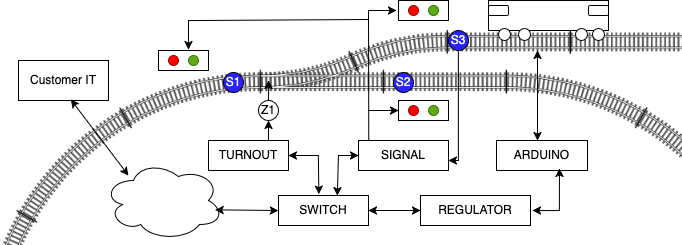
\includegraphics[height=20mm]{TrainSchema.png}
\end{wrapfigure}


From an Information Technology (IT) point of view, our system is shaped as shown on the right. Switches are controlled by a raspberry (TURNOUT) running an OpenPLC program, signals are controlled by an other raspberry, SIGNAL, with access to turnout positions via modbus. Then, the SIGNAL PLC reads mouvement sensors  (not all links shown in the figure) to update the status of signals. Next to that, we have a third machine, the regulator: it is in charge of updating train routes (as required by the customer IT),  of the regulation of turnouts and finally it may lock some signal (turn it to "red"). All the network connections are done via a single switch. Connections from REGULATOR to TURNOUT and SIGNAL are done via modbus while the customer IT and the regulator exchanges  are based on TCP/IP.  To be complete, to activate train mouvements, we use the DCC protocol via an Arduino, but this part is strictly related to the fact we have a train model. 


\begin{wrapfigure}[7]{r}{0.3\textwidth}
\hspace{-10mm}
 \begin{minipage}{0.3\textwidth}
        \centering
        \vspace{-24mm}
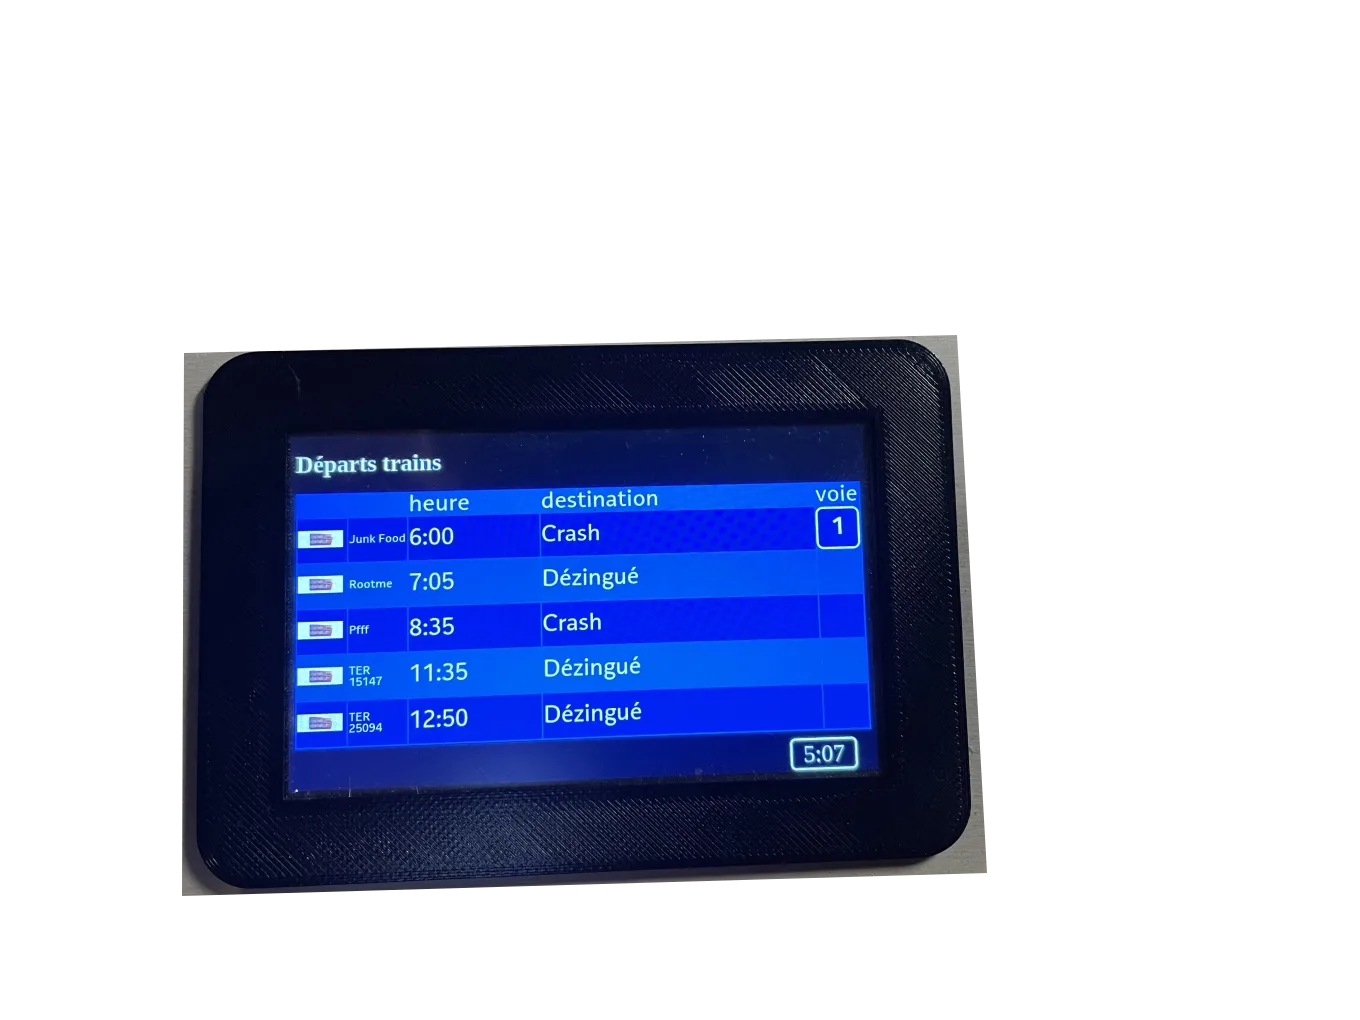
\includegraphics[height=50mm]{ZoomAffichage.png}
    \end{minipage}
\end{wrapfigure}

 The customer IT is deported from the infrastructure IT (thus the cloud).  It is itself composed of three machines: one for the station screens (on the right, after an attack), one for the databases and a final orchestrator. On the orchestrator, there are two main services: we have a web-service (with front and backend) and the general route scheduler.  Our model is completely automatic, no manual intervention is needed apart from minor electrical/mechanical problems that come with our scale model.
 
\begin{wrapfigure}[8]{r}{0.28\textwidth}
 \begin{minipage}{0.28\textwidth}
        \centering
        \vspace{-8mm}
\includegraphics[height=30mm]{maquette.png}
    \end{minipage}
\end{wrapfigure}

\paragraph{Final words on the N-scale model.} Our circuit has 8 blocks, 5 switches. Each block is bidirectional with a signal at each end. Blocks size goes from 25cm to 70cm.  We operate  three trains in parallel. Due to the size of the model, we reduced our signals  to "red" and "green" status, the trains being too close one from the other. Furthermore, in case of a red signal, we make the hypothesis that the train will be able to stop before it reaches the end of the block. In practice, we stop the trains in the middle. 

\paragraph{Routing trains.}
\todo{Ajouter: tout est automatique}
Routes are computed on the fly. The schedule is renewed every "day"\footnote{We use a time scale factor: one of our "day" corresponds to 20 minutes in real time.}  and we introduce some randomness in the process: beyond some routine daily planning, some trains are inserted/deleted, some trains departure/destination may change, and so on. We simulate also delays. Finally, in our model, we distinguish freight and  passengers routes giving priority to the latter. Routes are recomputed each time a train has finished its duty. The general motivation of this paper is to propose a lightweight scheduling solution that is adapted to the fully automatic control, that takes into account the distributed nature of the system, that is reliable and does not suffer from interlocking.  
 
We can now describe in more detail the working assumptions we are making about planning.  First, we have sensors on the rails at the two ends of each block. Accordingly,  we can catch train entrances within blocks. We make the hypothesis that this task is performed without errors. Second, the switches can be swapped from one position to the other, again, we suppose it is done without fault. Our method could cope such issues, but we leave that for future work. 
 
  Third, for trains, we have a simple policy.  According to its plan, a train may start in some direction (Forward/Backward) up to some final position. Then, once started, the train will run according to the signals: when green, it (re-)starts, when red, it stops.  We do not make hypotheses on the durations of travels, but once a train is running, it will reach in finite time the next block. Trains run in parallel independently. One train may enter a block, while an other is crossing some switch and the third one is breaking. There is no communications between the trains.

Fourth,  the regulator is capable of reading train block entrance events, requiring some switch swap and finally locking (that is make sure a signal is red)/unlocking some signal. We consider that those latter operations can be carried out without delay. Finally, the regulator may append some new duty to a train. To sum up, to control the train mouvements, the regulator can only lock/unlock signals. Naturally, a signal intended to block train $T_1$ may block $T_2$ if not set at the right time.   
 
 Parler de la stratégie, du modèle générale. All these operations are done by what we call  \emph{orders}. Roughly speaking, trains Orders have the shape "Start in direction Until position". Regulator orders are: \todo{en parler}. 
 
 
 To sum up, the regulation policy can be seen as an asynchronous distributed system. The N trains and the regulator are independent agents. That led us to TLA+, a framework introduced by Leslie Lamport for these kind of problems~\cite{Lamport}.  
 
\todo{ Comparaison avec les travaux antérieurs / lit review}
 
 
Due to the distributed nature of the regulation, building a safe policy can be very tricky. We want to show in this paper that tools from formal methods are very useful in this respect.  In this paper, we describe in  a first step the formalisation process. We go up to a TLA+ specification that will allow us checking two properties of route orchestration: safety and liveness. This is our first research question. 

Our second research question is the related to the following need. Suppose we want to append a new duty once a train reached its destination. This can be formalised as a composition problem (how to compose/concatenate some routes with some others). We describe such a composition procedure and then, again, we check that the routes are both safe and deadlock free. 

For our last research problem, we show that TLA+ may be used to refine a regulation policy. In our first attempts, we had typically some deadlocks issues. We have been able to detect them via TLA+ and then to provide some correction. 


% ############################# %
% Espace réservé aux encadrants %
% ############################# %


\subsection{Notations}

Given some set $S$ and some $x \not\in S$, we denote by $S_x = S \cup \{ x\}$.  An other notation: given some function $f: X \to Y$, $x \in X$ and $y \in Y$, we denote by $f[x \leftarrow y]$, the function:
 $$f[x \leftarrow y] \triangleq \left\{  \begin{array}{ll} x &\mapsto y\\
x' \neq x \in X &\mapsto f(x')
\end{array}\right.$$


\section{Model configurations}
\label{sec:informal-model}

In this section, we present configurations of our model, i.e. how we represent, at a given point in time, the state of our network. The dynamic rules of train routing are then presented in the following section.

Our model is has $k+1$ agents corresponding to the $k$ trains and the Regulator. Those agents take place on an infrastructure consisting of a track network equipped with signals. We first present the infrastructure model, then the agents.

\subsection{Infrastructure}

\paragraph{The network.} 

We suppose that the train network can be described as follows. First, we consider a set of $n$ blocks: $\blocks = \{ \bid{1}, \bid{2}, \ldots, \bid{n}\}$. Blocks are oriented: there is a $\dirForward$ (forward) end and a $\dirBackward$ (backward) one. Let $\directions = \{\dirForward, \dirBackward\}$ be the set of directions.  Second, we consider a set of $m$ trackworks\footnote{For the sake of simplicity, in this paper, we only consider switches. Our work can easily be extended to crossings and double slip switches (e.g. crossings have only one internal state and double slip switches have four states).}: $\turnouts = \{\sid{1}, \ldots, \sid{m}\}$. Trackworks are characterized by an internal state: switches can be in direct or deviate position (next denoted '\direct' and '\deviate'). Let $\internalState$ denotes the set of internal states. A \emph{network configuration} is given by a function $\sigma: \turnouts \to \internalState$. Let $\networkConf$ denotes the set of all network configurations. For instance, for two turnouts $\theta = \{\sid{1}, \sid{2}\}$, the function $\sid{1} \mapsto \deviate, \sid{2} \mapsto \direct$ states that switch $\sid{1}$ is in deviate position while \sid{2} is in direct one. The latter function is also described via an array  $[\deviate, \direct]$ giving states in trackwork order.

The network is then described as a triple $(\blocks, \turnouts, \sucblock)$ where $\sucblock$ is a partial function indicating the following block given a starting position, a direction and a network configuration: $\sucblock: \blocks\times \directions \times \networkConf \to \blocks$. We note $\suc{\bid{id}}{d}{\switches} = \nosuc$ when it is undefined. From an abstract point of view, the topology of the network reduces to that data.  


\paragraph{Signals.}
\todo{Est-ce qu'on met les signaux dans les agents ?}
At each end of the blocks, there is a signal whose state is \sigred (red) or \siggreen (green). In other words, the status of signals is described by a function $F: \blocks \times \directions \to \{ \sigred, \siggreen\}$. Given some signal status $F$, a block $\bid{id}$ and a direction $\dirFmt{d}$, $\signalF{\bid{id}}{d} = \sigred$ means the signal guarding the exit of block $\bid{id}$ in direction $\dirFmt{d}$ is red, and we expect trains not leaving that block going in this direction\footnote{Our semantics, presented in Section~\ref{sec:formal-model}, ensure such behaviour.}. The signal status is entirely determined by the network configuration and the locking status due to the regulator\todo{Le régulateur n'est pas encore introduit, je propose de déplacer ça plus bas.}.


\subsection{Agents}
\paragraph{Trains.}
We now present the train model. We consider a set of $k$ trains. 
Each train is characterised by an identifier, a position, a direction, and a list of orders.
\begin{itemize}
	\item Train identifiers form a set  $\trains = \{\tid{1}, \ldots, \tid{k}\}$, each train having its own identifier.
	\item The position is the index of the block currently occupied by the train.
	\item The direction (taken from $\directions_\dirStop = \{\dirBackward, \dirForward, \dirStop\}$) indicates the direction the train is ordered to go towards, where \dirStop indicates the train has no direction order at the moment. The direction represents the current move order, but does not mean the train is actually moving: it can be blocked at a signal.
	\item Orders are a (possibly empty) sequence of orders $\su{d}{\bid{1}\dots\bid{n}}$ ($\dirFmt{d} \in \directions$, $\bid{i} \in \blocks^\star$). Such order states that the train direction is set to $\dirFmt{d}$ and that the train will use blocks $\bid{1}\dots\bid{n}$.
\end{itemize}

Thus, each train is a quadruple $\trainFmt{t} = \trainTuple{\tid{id}}{\bid{id}}{d}{P}$ with $\tid{id}$ the train's identifier, $\bid{id}$ its position, $\dirFmt{d}$ its direction and $P$ its sequence of orders. Trains are collected in a sequence $\trainSeq = (\trainFmt{t_1}, \ldots, \trainFmt{t_k})$ where each $\trainFmt{t_i}$ being the tuple of train $\trainFmt{i}$. 


\paragraph{The Regulator.}
The regulator is in charge of the execution of the routing.
It is characterised by a routing program, a token list, and a waiting set.

\begin{itemize}
	\item The routing program $E$ specifies how the regulator should react to events (i.e. when a train enters a block). A program is a collection of rules to apply upon each event (called an \emph{event handler}). We detail further event handlers below.
	\item The token list, denoted $\tokens$, is a function  $\tokens: \blocks \to \Nat$ associating a token level to each block. Those tokens are used to prevent multiple trains accessing the same block at the same time.
	\item The waiting set is a set $W \subseteq \blocks \times \blocks \times \Nat \times \trains$. A triple $\tuple{\bid{src, }\bid{dst}, n, \tid{id}} \in W$ means that train \tid{id} is currently waiting in the block \bid{src} for $\tokenOf{\bid{id}}$ to be increased up to $n$.
\end{itemize}

Overall, the regulator is a tuple $R = \regTuple{E}{\tokens}{W}$. By convention, applying $\incr{pid}$ to the regulator is applying it to the token field: $R \cdot \incr{pid} = (E, T \cdot \incr{pid}, W)$. We use the same convention for the other atoms. \todo{move below}

\paragraph{Regulator's event handlers.}

Train events are handled by the regulator. Upon such events, the regulator can take actions such as turning a switch, allowing or blocking a train, etc.. The regulator is equipped with a routing program. This routing program contains, for each train, a list of handlers\todo{Chaque handler associe une position et une liste d'ordres.}. For a given train, the first handler of the list is the set of actions that have to be executed on the train's first event, second handler for the second event, and so on.

Given a routing program $E$, $\handlerOf{E}{\tid{id}}$ is the list of handlers of train $\tid{id}$, $\head{\handlerOf{E}{\tid{id}}}$ is the handler of the first event for that train.
The handler for a given event is a list of actions, each of them being one of the following:
\begin{description}
	\item [\wait{\bid{id}}{n}:] the train waits until the token of block \bid{id} reaches value $n$
	\item [\incr{\bid{id}}:] this increments the token $\bid{id}$ in $T$, thus releasing a train waiting
	\item [\turn{\sid{id}}{s}:] this turns the switch $\sid{id}$ into the $s$ state: $\sigma\cdot\turn{\sid{id}}{s} = \sigma[\sid{id} \leftarrow s]$
	\item [\auth:] a shortcut for waiting on oneself
\end{description}

Notice that all actions of a rule are executed atomically. Our semantics, presented below, details actions' behaviour.
\todo{Clarifier Event, indexation par train, qui donne une liste de handlers, eux-même une liste d'ordres}

\paragraph{Model.}
Overall, states of our model are tuples $\tuple{\trainSeq, \regulator, \switches, \signals}$ where $\trainSeq$ is a set of train tuples, $\regulator$ a regulator tuple, $\switches$ a network configuration (indicating trackworks states) and $\signals$ a signals state function. We suppose all train tuples in $\trainSeq$ have a different identifier. Notice that $\sucblock$ is not part of the state. Instead, the dynamics of the model (see below) is parameterised by $\sucblock$. Let $\modelSet$ be the set of all model states.

\paragraph{Network hypothesis, events, and conventions.}
On the tracks, we suppose there are sensors to detect the presence of trains. More precisely, we suppose that ---by means of the sensors--- the position of every train is known at any time. A \emph{position event} is when a train move from one block to an other one. 

Train speed are not modeled, and we consider trains can always stop within their current block if they have to (e.g. if there outgoing signal of a block is \sigred, we assume the train can stop in time).


\section{Model Semantics/Model dynamics}
\label{sec:formal-model}

In the previous section, we introduced our model. In this section, we present the dynamics of our model, that is the rules that govern how our model can switch from one state to the other.
We enrich our model with two elements: a guard, which goal is to schedule agents (for instance, it ensures the regulator acts atomically); and a communication buffer, which stores pending events until the regulator treats them. We present those two new elements in the first subsection.
The dynamics is described by means of a reduction relation, characterising the successive states of our model. We define this reduction relation using inference rules in the second subsection.

\todo{Expliquer le temps discret et le mix grand pas/petit pas.}

\subsection{Scheduling and communications}

In our dynamic rules, we distinguish three kinds of rules: one kind for trains, one kind for the regulator, and one kind for updating signals. We intend the signals' and regulator's reactions to be executed atomically. On the other hand, trains evolve much slower. To reflect this behaviour in our rules, we introduce a \emph{guard}. While, in our rules, the reaction of the regulator can take several steps, to implement atomic reaction, the guard blocks the rest of the system. Similarly, upon any train movement or regulator reaction, signals can be updated. In practice, such update happens instantly. To mimick this reaction of signal w.r.t. other events, the guard is in charge of blocking the system until signals are up-to-date.

Essentially, this guard is the state machine shown in Figure~\ref{fig:state_machine_guard}. The three states of the guard are \guardR, \guardS, and \guardT.

\begin{figure}
	\centering
	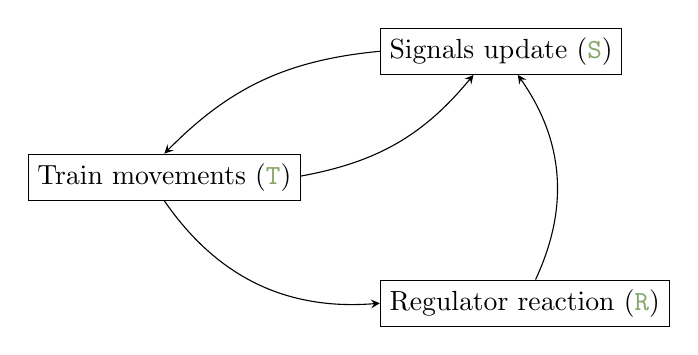
\begin{tikzpicture}
		\node[draw] (trains) {Train movements (\guardT)};
		\node[draw, above right=of trains] (signals1) {Signals update (\guardS)};
		\node[draw, below right=of trains] (regulator) {Regulator reaction (\guardR)};
		
		\draw[-stealth] (trains) to[bend right=20] (signals1);
		\draw[-stealth] (signals1.west) to[bend right=20] (trains.north);
		\draw[-stealth] (trains.south) to[bend right] (regulator.west);
		\draw[-stealth] (regulator) to[bend right] (signals1);
	\end{tikzpicture}
	\caption{State machine of the guard.}
	\label{fig:state_machine_guard}
\end{figure}

Train events are not dealt with instantly by the regulator (e.g. two train events can happen before the regulator begins to react to the first one). To characterise this behaviour, train events are stored in a buffer until the regulator uses them. In our model, a train event represent a train going from one block to another. When such thing happens, the train sends a message with its identifier to the regulator. A \emph{train buffer} \bufTrain is a sequence of such events, i.e. of train identifiers.
Similarly, the regulator communicates with signals with a \emph{signal buffer} \bufSig, which is a list of tuples $\tuple{\bid{id}, c}$, indicating that both signals of block $\bid{id}$ should be turned to color $c$. Let \bufTrainSet (resp. \bufSigSet) denote the set of train (resp. signal) buffers.

\subsection{Reduction rules}

States of the system are triples from $\{\guardR, \guardS, \guardT\} \times \bufTrainSet \times \bufSigSet \times \modelSet$. Our reduction relation is a binary relation on system states, noted $\reduces$: $S_1 \reduces S_2$ means that state $S_1$ can change to $S_2$ (note that this relation is not a function: $S_1$ can reduce to multiple states, due to non-determinism). We define $\reduces$ as the least relation induced by the inference rules presented hereafter.

\paragraph{Train rules.}
We first focus on rules that affect trains. The first rule is \ruleRef{Start}, which is used to change the direction of a train (e.g. to go from a stop to a given direction, or to change direction if the train has to backtrack). This rule can be triggered when the program of the train begins by \su{d^\prime}{N}. This order says that the train should got in direction $\dirFmt{d^\prime}$, and on that direction, it is expected to meet the sequence of block which ids are in $\posFmt{N}$.

\todo{Enlever les bid dans le buffer des trains}
\begin{mathpar}
	\inferrule*[left=\ruleDef{Start}]{
		\dirFmt{d} \neq \dirFmt{d^\prime} \and P = \trainConcat{\su{d^\prime}{\posFmt{N}}}{P^\prime}
	}{
		\hspace{3mm} \redTuple{\guardT}{\bufTrain}{\bufSig}{\stateTuple{\trainSeq{}\cup\{\trainTuple{\tid{id}}{\bid{id}}{d}{P}\}}{\regulator}{\switches}{\signals}} \\
		\reduces
		\redTuple{\guardT}{\push{\bufTrain}{\tuple{\tid{id}, \bid{id}}}}{\bufSig}{\stateTuple{\trainSeq{}\cup\{\trainTuple{\tid{id}}{\bid{id}}{d^\prime}{P}\}}{\regulator}{\switches}{\signals}}
	}
\end{mathpar}

Conversely, if the train program is empty (i.e. upon termination), the train stops using rule \ruleRef{Stop}.
\begin{mathpar}
	\inferrule*[left=\ruleDef{Stop}]{
		\dirFmt{d} \neq \dirStop
	}{
	\hspace{4mm}  \redTuple{\guardT}{\bufTrain}{\bufSig}{\stateTuple{\trainSeq{}\cup\{\trainTuple{\tid{id}}{\bid{id}}{d}{\emptyTrainProg}\}}{\regulator}{\switches}{\signals}} \\
	\reduces
	\redTuple{\guardT}{\push{\bufTrain}{\tuple{\tid{id}, \bid{id}}}}{\bufSig}{\stateTuple{\trainSeq{}\cup\{\trainTuple{\tid{id}}{\bid{id}}{\dirStop}{\emptyTrainProg}\}}{\regulator}{\switches}{\signals}}
	}
\end{mathpar}

The last two rules for trains describe what happens when a train actually moves, i.e. when its position changes. Two cases can occur, depending on the current order of the train: in \su{d}{N}, the $\posFmt{N}$ parameter is a list of blocks the train is about to encounter (including the current block), while going in direction \dirFmt{d}. Two cases occur, depending on whether \posFmt{N} contains future blocks or not. If \posFmt{N} contains only the upcoming block, then upon leaving the block, the order is removed (rule \ruleRef{UntilNext}); otherwise the upcoming block is simply popped from \posFmt{N} (rule \ruleRef{Until}). Notice that in both cases, the state of the guard changes to \guardS, meaning that signals will be updated immediately after that rule.\todo{Introduire/formaliser N} Also, both rules create an event, pushed in the buffer, informing the regulator that the train has changed block.

\begin{mathpar}
	\inferrule*[left=\ruleDef{Until}] {
		\suc{\bid{id}}{d}{\switches} = \bid{id^\prime} \neq \nosuc
		\and
		\signalF{\bid{id}}{d} = \siggreen
		\and
		\posFmt{N}\neq \varepsilon
	}{
		\redTuple{\guardT}{\bufTrain}{\bufSig}{\stateTuple{\trainSeq{}\cup\{\trainTuple{\tid{id}}{\bid{id}}{d}{\trainConcat{\su{d}{[\bid{id^\prime}; \posFmt{N}]}}{P}}\}}{\regulator}{\switches}{\signals}} \\
		\reduces		
		\redTuple{\guardS}{\push{\bufTrain}{\tuple{\tid{id}, \bid{id^\prime}}}}{\bufSig}{\stateTuple{\trainSeq{}\cup\{\trainTuple{\tid{id}}{\bid{id^\prime}}{d}{\trainConcat{\su{d}{[\posFmt{N}]}}{P}}\}}{\regulator}{\switches}{\signals}}
	}
\end{mathpar}

\begin{mathpar}
	\inferrule*[left=\ruleDef{UntilNext}] {
		\suc{\bid{id}}{d}{\switches} = \bid{id^\prime} \neq \nosuc
		\and
		\signalF{\bid{id}}{d} = \siggreen
	}{
		\redTuple{\guardT}{\bufTrain}{\bufSig}{\stateTuple{\trainSeq{}\cup\{\trainTuple{\tid{id}}{\bid{id}}{d}{\trainConcat{\su{d}{[\bid{id^\prime}]}}{P}}\}}{\regulator}{\switches}{\signals}} \\
		\reduces		
		\redTuple{\guardS}{\bufTrain}{\bufSig}{\stateTuple{\trainSeq{}\cup\{\trainTuple{\tid{id}}{\bid{id^\prime}}{d}{P}\}}{\regulator}{\switches}{\signals}}
	}
\end{mathpar}
Notice that, in \ruleRef{UntilNext}, no message is added to the buffer.
\todo{@Lucas, expliquer pourquoi c'est pas nécessaire.}

\paragraph{Regulator rules.}

When the regulator reacts to a train event, it executes atomically all rules associated with that event. To implement this atomic execution, the first regulator event is to change the guard to \guardR (see Fig. \ref{fig:state_machine_guard}).

\begin{mathpar}
	\inferrule*[left=\ruleDef{StartEvent}] {
		\buflen{B} \neq 0
	}{
		\redTuple{\guardT}{\bufTrain}{\bufSig}{R} \reduces \redTuple{\guardR}{\bufTrain}{\bufSig}{R}
	}
\end{mathpar}

Then, the regulator lookup the first event on the buffer, and executes all the rules in the event handler associated with this event. All actions are treated in order, and when the list of remaining actions is empty, the handling terminates and the event is removed of the buffer. We introduce 6 reduction rules for the 4 possible kinds of orders (\incr{\bid{id}} and \wait{\bid{id}}{i} have two rules).

Rule \ruleRef{Turn} triggers when a \turn{\sid{id}}{s} is encountered in the event handler. It updates the state of the targeted switch.
\begin{mathpar}
	\inferrule*[left=\ruleDef{Turn}]{
		\bufhead{B} = \tuple{\tid{id}, \bid{id}}
		\and
		\head{\handlerOf{E}{\tid{id}}} = \regConcat{\turn{\sid{id}}{s}}{A^\prime}
	}{
	\redTuple{\guardR}{\bufTrain}{\bufSig}{\stateTuple{\trainSeq}{\tuple{E, T, W}}{\switches}{\signals}}
	\reduces
	\redTuple{\guardR}{\bufTrain}{\bufSig}{\stateTuple{\trainSeq}{\tuple{\substHandlerHead{E}{\tid{id}}{A^\prime}, T, W}}{\updateSignals{\switches}{\sid{id}}{s}}{\signals}}
	}
\end{mathpar}

Of course, trains can conflict. For instance, if two trains have to use the same track, one has to go first and the other has to wait until the track is free. To schedule trains, we use a token system. Each block is assigned a token, which is an integer value. Trains can \emph{wait} until a token reaches a given value, and \emph{increment} a token after leaving a block. We introduce two pairs of rules for incrementing and waiting. The first pair deals with the case where the train waiting arrives before the token has the correct value, and the second pair deals with the (easier) case where the train releases the track (increments the associated token) before the next train arrives (and therefore does not need to wait).


To execute a \wait{\bid{critical}}{n} order, the regulator stores the train id in its waiting set, together with the current block of the train (\bid{src}), the block it is waiting for (\bid{critical}), and the value the token associated with the target block has to reach to release the train ($n$).
\begin{mathpar}
	\inferrule*[left=\ruleDef{WaitBefore}] {
		\bufhead{B} = \tuple{\tid{id}, \bid{id}}
		\and
		\head{\handlerOf{E}{\tid{id}}} = \regConcat{\wait{\bid{critical}}{n}}{A^\prime}
		\\
		\tokenOf{\bid{critical}} \neq n
	}{
		\redTuple{\guardR}{\bufTrain}{\bufSig}{\stateTuple{\trainSeq}{\tuple{E, T, W}}{\switches}{\signals}}
		\\\reduces
		\redTuple{\guardR}{\bufTrain}{\bufSig}{\stateTuple{\trainSeq}{\tuple{\substHandlerHead{E}{\tid{id}}{A^\prime}, T, W\cup\tuple{\bid{src}, \bid{critical}, n, \tid{id}}}}{\switches}{\signals}}
	}
\end{mathpar}

Then, when the releasing train frees the critical block, the token is incremented, and the train waiting for the new value of the token is released\footnote{By construction, nothing prevents multiple trains to be waiting for the same value, thus resulting in a faulty system. However, our model checker ensures programs (including event handlers) are correct, thus detecting such case.} and updates the signals to let the waiting train go.

\begin{mathpar}
	\inferrule*[left=\ruleDef{IncrAfter}] {
		\bufhead{B} = \tuple{\tid{id}, \bid{id}}
		\and
		\head{\handlerOf{E}{\tid{id}}} = \regConcat{\incr{\bid{critical}}}{A^\prime}
		\\
		\exists \bid{src}, \tid{waiting} \text{ s.t. } \tuple{\bid{src}, \bid{critical}, \tokenOf{\bid{critical}} + 1, \tid{waiting}} \in W
		\\
		\nextWait{\handlerOf{E}{\tid{waiting}}} = \bid{next\_stop}
	}{
		\redTuple{\guardR}{\bufTrain}{\bufSig}{\stateTuple{\trainSeq}{\tuple{E, T, W}}{\switches}{\signals}}
		\\\reduces
		\redTuple{\guardR}{\bufTrain}{\bufSig}{\stateTuple{\trainSeq}{\tuple{\substHandlerHead{E}{\tid{id}}{A^\prime}, T[\bid{critical} \leftarrow T(\bid{critical})+1], W\setminus\{\tuple{\bid{src}, \bid{critical}, \tokenOf{\bid{critical} + 1}, \tid{waiting}}\}}}{\switches}{\signals}}
	}
\end{mathpar}
\todo{ajouter $\tuple{\bid{next\_stop, \sigred}}, \tuple{\bid{src}, \siggreen}$}
\todo{expliquer \nextWait{E}}

On the other hand, if the releasing train arrives before the waiting train, the increase rule does not need to modify the waiting set (as the waiting train is not yet in it), nor the signals\footnote{The upcoming red signal of the waiting train is dealt with in the dual \ruleRef{WaitAfter} rule.}. It only needs to increase the token. This case is detected by looking at the waiting set, when it contains no waiting train with the new value.


\begin{mathpar}
	\inferrule*[left=\ruleDef{IncrBefore}] {
		\bufhead{B} = \tuple{\tid{id}, \bid{id}}
		\and
		\head{\handlerOf{E}{\tid{id}}} = \regConcat{\incr{\bid{critical}}}{A^\prime}
		\\
		\neg\exists \bid{src}, \tid{waiting} \text{ s.t. } \tuple{\bid{src}, \bid{critical}, \tokenOf{\bid{critical}} + 1, \tid{waiting}} \in W
	}{
		\redTuple{\guardR}{\bufTrain}{\bufSig}{\stateTuple{\trainSeq}{\tuple{E, T, W}}{\switches}{\signals}}
		\\\reduces
		\redTuple{\guardR}{\bufTrain}{\bufSig}{\stateTuple{\trainSeq}{\tuple{\substHandlerHead{E}{\tid{id}}{A^\prime}, T[\bid{critical} \leftarrow T(\bid{critical})+1], W}}{\switches}{\signals}}
	}
\end{mathpar}

Then, when the waiting train arrives, instead of stopping the train, the regulator can update the signal and let it continue until its next waiting point. This case is identified when the token already has the value the train expects\footnote{Notice that if the train misses its slot, e.g. if an incorrect program increases twice the token, the train will not continue, as another train, waiting for the twice-increased value, might be on the tracks.}.
\begin{mathpar}
	\inferrule*[left=\ruleDef{WaitAfter}] {
		\bufhead{B} = \tuple{\tid{waiting}, \bid{id}}
		\and
		\tokenOf{\bid{critical}} = n
		\\
		\nextWait{\handlerOf{E}{\tid{waiting}}} = \bid{next\_stop}
		\and
		\head{\handlerOf{E}{\tid{id}}} = \regConcat{\wait{\bid{critical}}{n}}{A^\prime}
	}{
		\redTuple{\guardR}{\bufTrain}{\bufSig}{\stateTuple{\trainSeq}{\tuple{E, T, W}}{\switches}{\signals}}
		\reduces
		\redTuple{\guardR}{\bufTrain}{\bufSig}{\stateTuple{\trainSeq}{\tuple{\substHandlerHead{E}{\tid{id}}{A^\prime}, T, W}}{\switches}{\signals}}
	}
\end{mathpar}
\todo{M-à-J des feux}

\begin{mathpar}
	\inferrule*[left=\ruleDef{Auth}] {
		\bufhead{E[\tid{id}]}.pos = \bid{id}
		\and
		\bufhead{B} = \tuple{\tid{id}, \bid{id}}
		\\
		\nextWait{\buftail{E[\tid{id}]}} = \bid{wait}
		\and
		\head{\handlerOf{E}{\tid{id}}} = \regConcat{\auth}{A^\prime}
	}{
			\redTuple{\guardR}{\bufTrain}{\bufSig}{\stateTuple{\trainSeq}{\tuple{E, T, W}}{\switches}{\signals}}
			\reduces
			\redTuple{\guardR}{\bufTrain}{\bufSig}{\stateTuple{\trainSeq}{\tuple{\substHandlerHead{E}{\tid{id}}{A^\prime}, T, W}}{\switches}{\signals}}
	}
\end{mathpar}\todo{ajouter $\tuple{\bid{wait}, \sigred}, \tuple{\bid{id}, \siggreen}$ dans le buffer des signaux}
where \nextWait{E} returns the next position (block id) where the train has to was, using the event handlers of the train in question. Notice that, in our case, we consider the tail of the event handlers of the train, since it is already waiting and we want the next waiting location. \todo{rephrase}

\todo{other rules}

Finally, when the handler of the pending event has no action leftover, the regulator terminates its handling: it removes the (now empty) head of $\handlerOf{E}{\tid{id}}$, the head of the buffer, and returns the guard to state $\guardT$.

\begin{mathpar}
	\inferrule*[left=\ruleDef{EndEvent}]{
		\bufhead{B} = \tuple{\tid{id}, \bid{id}}
		\and
		\head{\handlerOf{E}{\tid{id}}} = \emptyList
	}{
		\redTuple{\guardR}{\bufTrain}{\bufSig}{\stateTuple{\trainSeq}{\tuple{E, T, W}}{\switches}{\signals}}
		\reduces
		\redTuple{\guardS}{\buftail{\bufTrain}}{\bufSig}{\stateTuple{\trainSeq}{\tuple{\popHandlerHead{E}{\tid{id}}, T, W}}{\switches}{\signals}}
	}
\end{mathpar}

\paragraph{Signal rules.}



\paragraph{Guillaume rajoute la normalisation}

%Rule application induce a relation between system state:  $S\reduces S'$ if $\gamma'$  if there is a rule for which $\gamma$ is the initial state and $\gamma'$ the conclusion. 
The reflexive-transitive closure of $\reduces$ is denoted $\reduces^*$, that is $S \reduces^* S'$ iff $S =S_0 \reduces \cdots S_n = S'$. The value $n = 0$ corresponds to $S = S'$.  A normal form of a configuration $S$ is a configuration $S'$ such that $S \reduces^* S'$ and there is no $S''$ with $S' \reduces S''$. In other words, starting from $S$, the computation can stop on $S'$. We note $S \reduces^! S'$ this relationship.

Given a system state  $S = \redTuple{x}{\bufTrain}{\bufSig}{\stateTuple{\trainSeq{}}{\regulator}{\switches}{\signals}}$ and a train $\tid{id}$, 
\begin{itemize}
	\item   we say that it has no jobs if  $\trainSeq{}[\tid{id}].P = \emptyTrainProg$;
	\item its source is $\mathtt{src}(S, \tid{id}) = \trainSeq{}[\tid{id}].pid$;
	\item its destination is $\mathtt{dst}(S, \tid{id}) = pid \in \blocks $ if either
	\begin{itemize}
		\item  it has no jobs and  $\trainSeq{}[\tid{id}].pid = pid$  or
		\item  the last order in  $\trainSeq{}[\tid{id}].P$ is $\su{d}{pid}$ for some direction $d$.
	\end{itemize}
\end{itemize}

A system state $S = \redTuple{\guardT}{\emptyset}{\bufSig}{\stateTuple{\trainSeq{}}{\regulator}{\switches}{\signals}} $  is \emph{reliable} if: 
\begin{itemize}
	\item  no two trains meet on the same block or the same switch, \todo{En dire plus}
	\item $S$ has  a unique normal form $S'$ and 
	\item any train in $S'$ has no jobs and 
	\item for any train $\tid{id}$, $\mathtt{dst}(S, \tid{id}) =  \mathtt{dst}(S', \tid{id})$. 
\end{itemize}

\subsection{Détecter les problèmes}
Cette section est particulièrement importante, modéliser les problèmes que l'on peut rencontrer permet de les détecter.
Cette phrase peut paraître évidente, mais elle est centrale dans notre méthodologie. Ici, nous pouvons faire face à deux problèmes : 
les trains n'arrivent pas destination, c'est un deadlock, ou les trains partagent une même ressource, c'est un crash. 
Point important, nos règles de transitions se basent sur l'interleaving, les trains ne peuvent donc pas se croiser. (($\triangle$,2) $\Rightarrow$ ($\triangle$,3) || ($O$,3) $\Rightarrow$ ($O$,2)).
Le premier problème représente notre propriété de Liveness, les trains arrivent à destination, et le second représente notre propriété de Safety, les trains ne se crashent pas.

\section{Formalisation within TLA+}
\label{sec:tla-formalisation}

Our global aim is to check that routes are correct. That is we want, for any initial configuration, to check that no trains meet on the same block, that there is no deadlocks and finally  that trains will reach their destination. To do that, we implement the rules of Section~\ref{sec:formal-model} in TLA+. The tool provides both a specification language and a model checker. We let the reader refer to the book of Lamport~\cite{Lamport} for a full presentation of TLA+. 

To specify a system in TLA+, first, a configurations is described as a list of variables, then rules  will give the dynamic of the system and finally some assertions  will check the model.  Variables values range within sets. Either directly, or via a library, we have access to integers, strings, finite sets (e.g. \mintinline{C}{ T = {1, 2, 3}}), sequences (e.g. \mintinline{C}{route = <<7,3,4>>}),  arrays (e.g. for the initial token valuation \mintinline{C}{token = [bid in 1..nbBlock |-> 0]} ) and tuples (e.g. \mintinline{C}{[tid|->1, pid|->9, d|->"*", prog|-> << <<"StartUntil","f",4>> >>]}  for a train configuration:).

With those latter constructions, we can represent an initial configuration. It takes the form of a logical formula (partially given here):
\begin{minted}{C}
Init == 
    LET 
        four_to_8 ==  << <<"StartUntil","b",<<3,8>> >>  >>
        five_to_4 ==  << <<"StartUntil","f",<<7,3,4>> >> >>
        train1 == [tid|->1, pid|->4, d|->"*", prog|-> four_to_8]
        train2 == [tid|->2, pid|->5, d|->"*", prog|-> five_to_4]
        traffic_lights ==[x \in (1..8) \X {"f","b"} |-> "g"]
        ...
    IN
        /\ gamma = <<train1,train2>>
        /\ sigma =  <<"d", "d", "v", "d", "d">> 
        /\ F = [traffic_lights EXCEPT ![7,"f"]="r", ![8,"b"]="r"]
        ...
\end{minted}

The representation of the network topology is also represented within TLA+. It takes the shape of a function that is precomputed via a python script (see XXX\todo{Référence au schéma}). 

\subsection{The implementation of the dynamics}

Variables will be updated with time flying, each transition is described with prime variables. Those latter represent the value of the variable after the transition. For instance, \mintinline{C}{gamma' = [gamma EXCEPT ![T.id].d = "*"]} updates the train tuple: the train \mintinline{C}{T.id}'s direction is set to \mintinline{C}{"*"} where  \mintinline{C}{T} is a variable  defined somewhere else. 

To each inference rule in Section~\ref{sec:formal-model}, we associate a TLA+ rule taking the shape (here the Stop rule): 
\begin{minted}{C}
Stop (T) ==
        /\ Len(T.prog) = 0
        /\ meta.G.state = "none"
        /\ T.d /= "*"
        /\ gamma' = [gamma EXCEPT ![T.id].d = "*"]
        /\ meta' = [meta EXCEPT !.msg[1] = Append(meta.msg[1],<<T.id,T.pid>>)]
        /\ UNCHANGED << reg, sigma, F >>
 \end{minted}
The first three lines correspond to the conditions that will fire the rule, the last ones correspond to the configuration update. The next definition represent the application of one rule:
\begin{minted}{C}
Next == 
   \/ UpdateTL
   \/ StartEvent
   \/ Turn
   ...
   \/  \E i \in 1..Len(gamma) :
            \/ Stop(gamma[i])
            \/ Until(gamma[i])
            ...
\end{minted}       
        
The system is then represented by a formula:
\begin{verbatim}
    Spec == Init /\  [][Next]_variables
\end{verbatim}%Revoir la syntaxe au cas où / remplacer par le jolie tla2latex
where variables is the tuple of all variables. The intended meaning is that the initial configuration is specified in \mintinline{C}{Init} and steps follow the \mintinline{C}{Next} formula.  Actually, presently, in our formal semantics, nothing forces a rule to be applied. As a consequence, an ongoing train may never reach its next block. Thanks to TLA+, we can ensure that a rule will eventually be applied (if it can be). Those are known as weak fairness conditions. Again, we specify it as follows. \todo{WF condition?}


\section{Composition}
\label{sec:composition}

The main principle behind our scheduling process is based on the notion of route. A route for a train is a sequence $\vec{x} = x_1, \ldots, x_k$ of (contiguous) blocks and switches starting and ending on a block.   Two routes $\vec{x}$ and $\vec{y}$ have a critical resource if  $x_i = y_j$ for some $i,j$. A \emph{global routing}, denoted $X = (\vec{x}^{id})_{id \in \trains}$,  is a route for each train. Informally, a \emph{safe step} is a global routing such that there are no critical resources between two routes and there is a network configuration $\sigma$ such that  for each train $\tid{id}$, there is a direction according to which starting at $x_1^{id}$, following that direction and given the configuration $\sigma$, one reaches $x_{k_{id}}^{id}$. Let us turn to the technical definition.   A safe step is a global routing $X$ such that:
\begin{itemize}
\item for any $\tid{id} \neq \tid{id'} \in \trains$, $\vec{x}^{id}$ and $\vec{x}^{id'}$ have no critical resources,
\item for any $\tid{id} \in \trains$, there is a privileged pair $\langle d, \sigma\rangle$  for $\vec{x}^{id}$,
\item all the privileged pairs share the same value $\sigma$. 
\end{itemize}

Given a route $\vec{x} = x_1, \ldots, x_k$, we say that $\vec{x}$ has a privileged pair $\text{priv}(\vec{x}) = \langle d, \sigma\rangle \in \directions \times \Sigma$ whenever for any pair $i < j$ such that
\begin{itemize}
\item  $x_i$, $x_j$ are blocks and  , 
\item $x_{i+1}, \ldots, x_{j-1}$ are switches
\end{itemize} 
then  $\sucblock(x_i, d, \sigma) = x_j$.


Any global routing can be seen as the composition of safe steps and actually, that provides a scheduling algorithm. We say that a sequence of positions $(\bid{id})_{id \in \trains}$ is \emph{separate} if there are no two trains $\tid{id} \neq \tid{id'}$ with $\bid{id} = \bid{id'}$. This notion induces a graph: let $G = \langle V, E\rangle$ with $V$ the set of separate positions and $E$ the set of safe steps between them.  Then, to compute global routes, we look for a path in the graph from the source to the target. The  $A^*$ algorithm we implemented is proving highly effective. This strategy has a main advantage, it is quite flexible with respect to new events. Suppose that at some point a train is blocked, we may recompute safe steps for the other trains, possibly releasing a deadlock. 

 But, that being said, we are now turned to the transformation of safe steps into system states, that is train orders and regulator rules. And then, to compose those system states into global routes. 

\subsection{Safe steps}
\label{sec:experiments:4}

To each safe step $X = (\vec{x}_i)_{i \in \trains}$, we can associate a system state $C(X) = \redTuple{\guardG}{\bufferFmt{B}}{\stateTuple{\trainSeq}{\regulator}{\switches}{\signals}} $ as follows. 
\begin{itemize}
\item $\guardG = \guardT$,
\item $\bufferFmt{B} = \emptyList$,
\item for each train $\tid{id}$, $\trainSeq[id] = \trainTuple{\tid{id}}{\bid{id}}{d}{\su{d}{x^{id}_{k_{id}}}}$ with $\langle d,\sigma\rangle = \text{priv}(\vec{x}^{id})$,
\item $R = \langle E, 0, \emptyset\rangle$, $E$ being defined below,
\item $\sigma$ is the unique network configuration shared by all privileged pairs (here we suppose that there is at least one(!) train),
\item $F = \blocks \times \directions \to \{\sigred, \siggreen \}$:
$$
(\bid{id}, d) \mapsto \left \{ \begin{array}{ll}
\sigred & \text{if } \exists \tid{id} \in \trains \text{ such that }  \bid{id} = x^{id}_{k_{id}} \text{ and } \langle d,\sigma\rangle = \text{priv}(\vec{x}^{id}) \\
\siggreen & \text{otherwise}
\end{array} \right.$$
\end{itemize}

\todo{ La notion de priv(x) dit qu'il est unique.}

With TLA+, we checked that any safe step is actually reliable.  On our network, one finds 58 368 safe steps, all being reliable. Checking all the path took XXX seconds on YYY. \todo{XXX= nombre de seconde, YYY = décrire la machine (processeur, RAM, etc)}

%\subsection{Test sur les chemins élémentaires}

%Avant de passer à la composition, nous devons tester que l'algorithme permettant de "parser" un chemin élémentaire en TLA+ depuis sa description contenue dans le fichier JSON fonctionne.
%Pour cela, nous allons tester les 165 500 chemins élémentaires de notre circuit, du moins, ceux que l'on considère comme "valides".
%Certains chemins élémentaires ne font que démarrer, ce qui n'a pas de sens dans notre modèle, aucune règle de transition n'est prévue pour cela.
%Après 111 812 secondes, soit 31 heures, l'intégralité des chemins a été passée en revue. Parmi eux, 58 368 chemins valides ont été testés, ne rencontrant aucun problème. (Sur l'image on lit 58 370, petit bug d'affichage que j'ai laissé passer)  

\begin{figure}
	\begin{subfigure}{0.5\textwidth}
		\centering
		%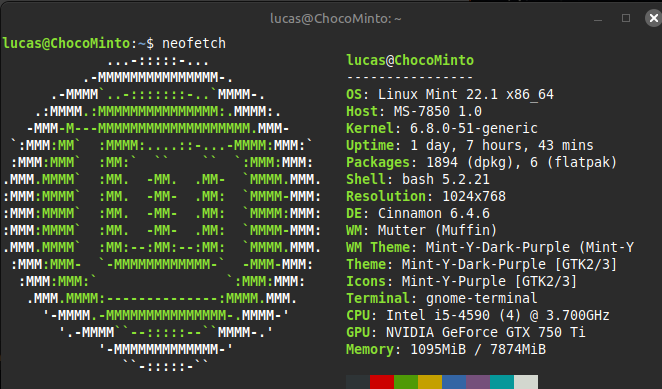
\includegraphics[width=\textwidth]{img/spec_pc.png}
		\caption{Spec de l'ordinateur}
	\end{subfigure}
	\begin{subfigure}{0.5\textwidth}
		\centering
		%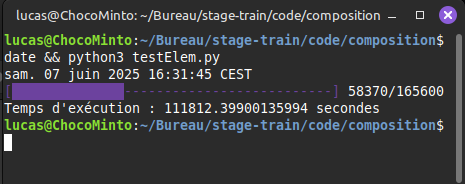
\includegraphics[width=\textwidth+0.5cm]{img/testElem.png}
		\caption{Vérification des chemins élémentaires}
	\end{subfigure}
	\caption{Tests sur les chemins élémentaires}
\end{figure}
\label{fig:elem-tests}


\subsection{Safe steps composition}

Two states $S$ and $S'$ are said to be \emph{compatible} whenever:
\begin{itemize}
\item for any train $\tid{id}$, we have $\mathtt{dst}(S, \tid{id})  =  \mathtt{src}(S', \tid{id})$,
\item for any normal form $S \reduces^! S''$, we have $S''.\sigma = S'.\sigma$.
\end{itemize}
In other words, at the arrival of $S$, trains are at the starting position of $S'$ and so are switches. We define the composition on compatible states. Actually, we describe composition of a system state and a safe step. So, from the remaining of the section, we suppose $S$ and $S'$ be compatible state, $S'$ being a safe step. We aim to compute their composition $S''  = \redTuple{x}{\bufTrain}{\bufSig}{\stateTuple{\trainSeq}{\regulator}{\switches}{\signals}}$.

\paragraph{Train composition} For each train $\tid{id}$, the composition of $S$ and $S'$ is: $S''.\stateTuple[\tid{id}] = \langle S.\stateTuple[\tid{id}].pid$, 



\subsection{Preparation}

The first step is the computation of critical resources. A block $\bid{id}$ is said to be critical if it occurs in both a train sequence in $S$ occurs an other train sequence in $S'$. A switch $\sid{id}$ is said to be critical if it occurs in one order of the regulator $S.R$ and in one order of $S'.R$. 



%\textbf{Simplification des ordres "turn"}\\
%La préparation est une étape cruciale, nous permettant de simplifier la suite du processus.
%D'abord, nous allons simplifier les ordres "turn", pour cela, {\color{red} on pose l'hypothèse que o1 et o2 sont élémentaires (embêtant si on veut faire des compositions complexes)}.
%Ainsi, dans chaque liste d'ordre, un ordre "turn" ne peut concerner qu'un seul switch. On cherche alors les ordres similaires entre les listes pour les supprimer de o2.
%\\Par exemple :

%\begin{center}
%	\begin{tabular}{||c || c | c||}
%		\hline
%		tid & o$_1$ & o$_2$ \\ [0.5ex] 
%		\hline\hline
%		0 & \tuple{10d,{\color{blue}11v}} & \tuple{} \\ 
%		1 & \tuple{} & \tuple{{\color{blue}12v},10d} \\
%		\hline
%		0 & \tuple{{\color{blue}10d},11v} & \tuple{} \\ 
%		1 & \tuple{} & \tuple{{\color{blue}12v},10d} \\
%		\hline
%		0 & \tuple{10d,{\color{violet}11v}} & \tuple{} \\ 
%		1 & \tuple{} & \tuple{12v,{\color{violet}10d}} \\
%		\hline
%		0 & \tuple{\underline{\color{violet}10d},11v} & \tuple{} \\ 
%		1 & \tuple{} & \tuple{12v,\underline{\color{violet}10d}} \\
%		\hline
%		0 & \tuple{10d,11v} & \tuple{} \\ 
%		1 & \tuple{} & \tuple{12v} \\
%		\hline
%	\end{tabular}
%\end{center}
%On convertie ensuite les ordres "turn" restant dans o1 en "initialisation" d'un aiguillage si ce dernier n'est pas déjà initialisé.
%\\\textbf{Traiter les ressources critiques}\\
%Pour cette étape, on cherche d'abord à identifier les ressources critiques. Avec une méthode similaire à celle vue précédemment :

%\vspace{0.5cm}

%\begin{center}
%	\begin{tabular}{||c || c | c||} 
%		\hline
%		tid & o$_1$ & o$_2$ \\ [0.5ex] 
%		\hline\hline
%		0 & \tuple{4,3,{\color{red}8}} & \tuple{8} \\ 
%		1 & \tuple{6} & \tuple{{\color{red}7},3,4,5} \\
%		\hline
%		0 & \tuple{4,{\color{red}3},8} & \tuple{8} \\ 
%		1 & \tuple{6} & \tuple{{\color{red}7},3,4,5} \\
%		\hline
%		0 & \tuple{{\color{red}4},3,8} & \tuple{8} \\ 
%		1 & \tuple{6} & \tuple{{\color{red}7},3,4,5} \\
%		\hline
%		
%		0 & \tuple{4,3,{\color{violet}8}} & \tuple{8} \\
%		1 & \tuple{6} & \tuple{7,{\color{violet}3},4,5} \\
%		\hline
%		0 & \tuple{4,\underline{\color{violet}3},8} & \tuple{8} \\ 
%		1 & \tuple{6} & \tuple{7,\underline{\color{violet}3},4,5} \\
%		\hline
%
%		0 & \tuple{4,3,{\color{blue}8}} & \tuple{8} \\
%		1 & \tuple{6} & \tuple{7,3,{\color{blue}4},5} \\
%		\hline
%
%		0 & \tuple{4,3,{\color{orange}8}} & \tuple{8} \\
%		1 & \tuple{6} & \tuple{7,3,4,{\color{orange}5}} \\
%		\hline
%	\end{tabular}
%\end{center}
\noindent
Dans notre exemple, on peut voir que 3 est la seule ressource critique, il faut donc traiter ce cas.
On va ajouter un ordre "att(3,valT)" à l'event précédent l'entrée de la ressource critique pour le train qui utilise la ressource en second.
On ajoute également un ordre "incr(3)" à l'event suivant la sortie de la ressource critique pour le train qui utilise la ressource en premier.
Si le train à besoin d'un "turn" pour entrer dans la ressources critique, alors on le décale dans un event du train ayant utilisé l'aiguillage le plus récemment.
\\\textbf{Mettre à jour les jetons}\\
Laissons de côté l'hypothèse que o1 et o2 sont élémentaires, il est alors possible que o1 contienne des ordres de type "att" et "incr". Il faut donc mettre à jour les valeurs
des tokens pour "att" et "incr" dans o2. Par exemple, si dans o1 on trouve les ordres : (att(3,1), incr(3)), alors dans o2 on va devoir transformer att(3,1) en att(3,2).

\subsection{Assemblage}
L'assemblage est la partie la plus simple de cette fonction, il s'agit de concaténer les ordres des trains et des events.
Pas de technique intelligente, si les programmes du train 1 pour o1 et o2 sont "<L,[1,2]>" et "<L,[3,4]>", alors la concaténation donne "<L,[1,2]>,<L,[3,4]>".
Même chose pour les events, \tuple{\tuple{1,\tuple{}},\tuple{2,\tuple{turn(x,y)}}} et \tuple{\tuple{2,\tuple{att(3,1)}},\tuple{3,\tuple{}}} devient \tuple{\tuple{1,\tuple{}},\tuple{2,\tuple{turn(x,y),(att(3,1))}},\tuple{3,\tuple{}}}.
À partir de maintenant, nous ne manipulerons plus deux listes d'ordres, o1 et o2, mais une seule : o3. 
\\Aussi, on reprend l'initialisation des aiguillages de o1 pour o3.

\subsection{Nettoyage}
Cette partie fait office de "finalisation". On va d'abord s'occuper de "regrouper" les ordres des trains. Notre exemple précédent "<L,[1,2]>,<L,[3,4]>", nous donne maintenant "<L,[1,2,3,4]>". 
On ajoute également un ordre "auth" pour les "turn" utilisés par des trains pour agir sur leur propre parcours. (les trains n'utilisent pas directement "turn", mais plus simple à expliquer de cette manière)
Enfin, on chercher le premier arrêt de chaque train pour assigner les feux au rouge.

Maintenant que tous les éléments sont définis, nous pouvons nous intéresser à la vérification de notre modèle.
L'ultime but est de tester tous les chemins possibles sur notre modèle pour s'assurer qu'il est correct pour n'importe quel chemin.
Ce projet est ambitieux, nous allons donc nous concentrer sur la composition de deux chemins élémentaires, et vérifier que le modèle est correct pour ces cas.


\subsection{Experiments}
\label{sec:experiments:4}


\section{Conclusion}
\label{sec:conclusion}

\paragraph{Contributions.}
This paper introduces three main contributions. First we presented a formal model for railway network. Our model simplifies multiple elements from real life networks, but nonetheless keeps non-trivial elements, such as trackworks and signals. Contrary to existing models, ours makes very few assumptions about the network: tracks are two ways and \todo{...}

Our second contribution is the implementation of our model in the TLA+ model checker. Our implementation allows to verify that routing schedules are free from deadlocks and crashes, and reaches correct destinations. We tested our implementation on various schedules on a small-scale network, where the computation time was found to be negligible. Our implementation takes approximately 500 lines of TLA+.

Our third contribution is a composition operator. This operator allows to incrementally build routing schedules, which can then be tested using our TLA+ implementation. Our composition distinguishes safe steps: steps where no two trains use the same track. Our composition can append safe steps to arbitrary schedules, creating new schedules. We implemented our composition operator in Python and we tested it by model checking all schedules composed of two and three safe steps in our small-scale network. The computation time was found to be affordable for companies: checking all two-steps schedules took less than a day on a cluster, using 8 nodes of 18 cores.

Our implementation, including both the TLA model and the Python composition is available on...\todo{Donner le lien vers github ? }.

\paragraph{Limitations and future works.}
The main limitation of our paper regards scaling our approach. While we tested extensively our implementation on small-scale systems (small network, few trains), we expect the number of state to explode on larger networks. We intend to perform larger tests in future work.

\todo{On peut avoir des routages de n'importe où, donc on peut voir pour interfacer avec d'autres approches ?}

%temporaire, histoire d'avoir le sommaire en tête
%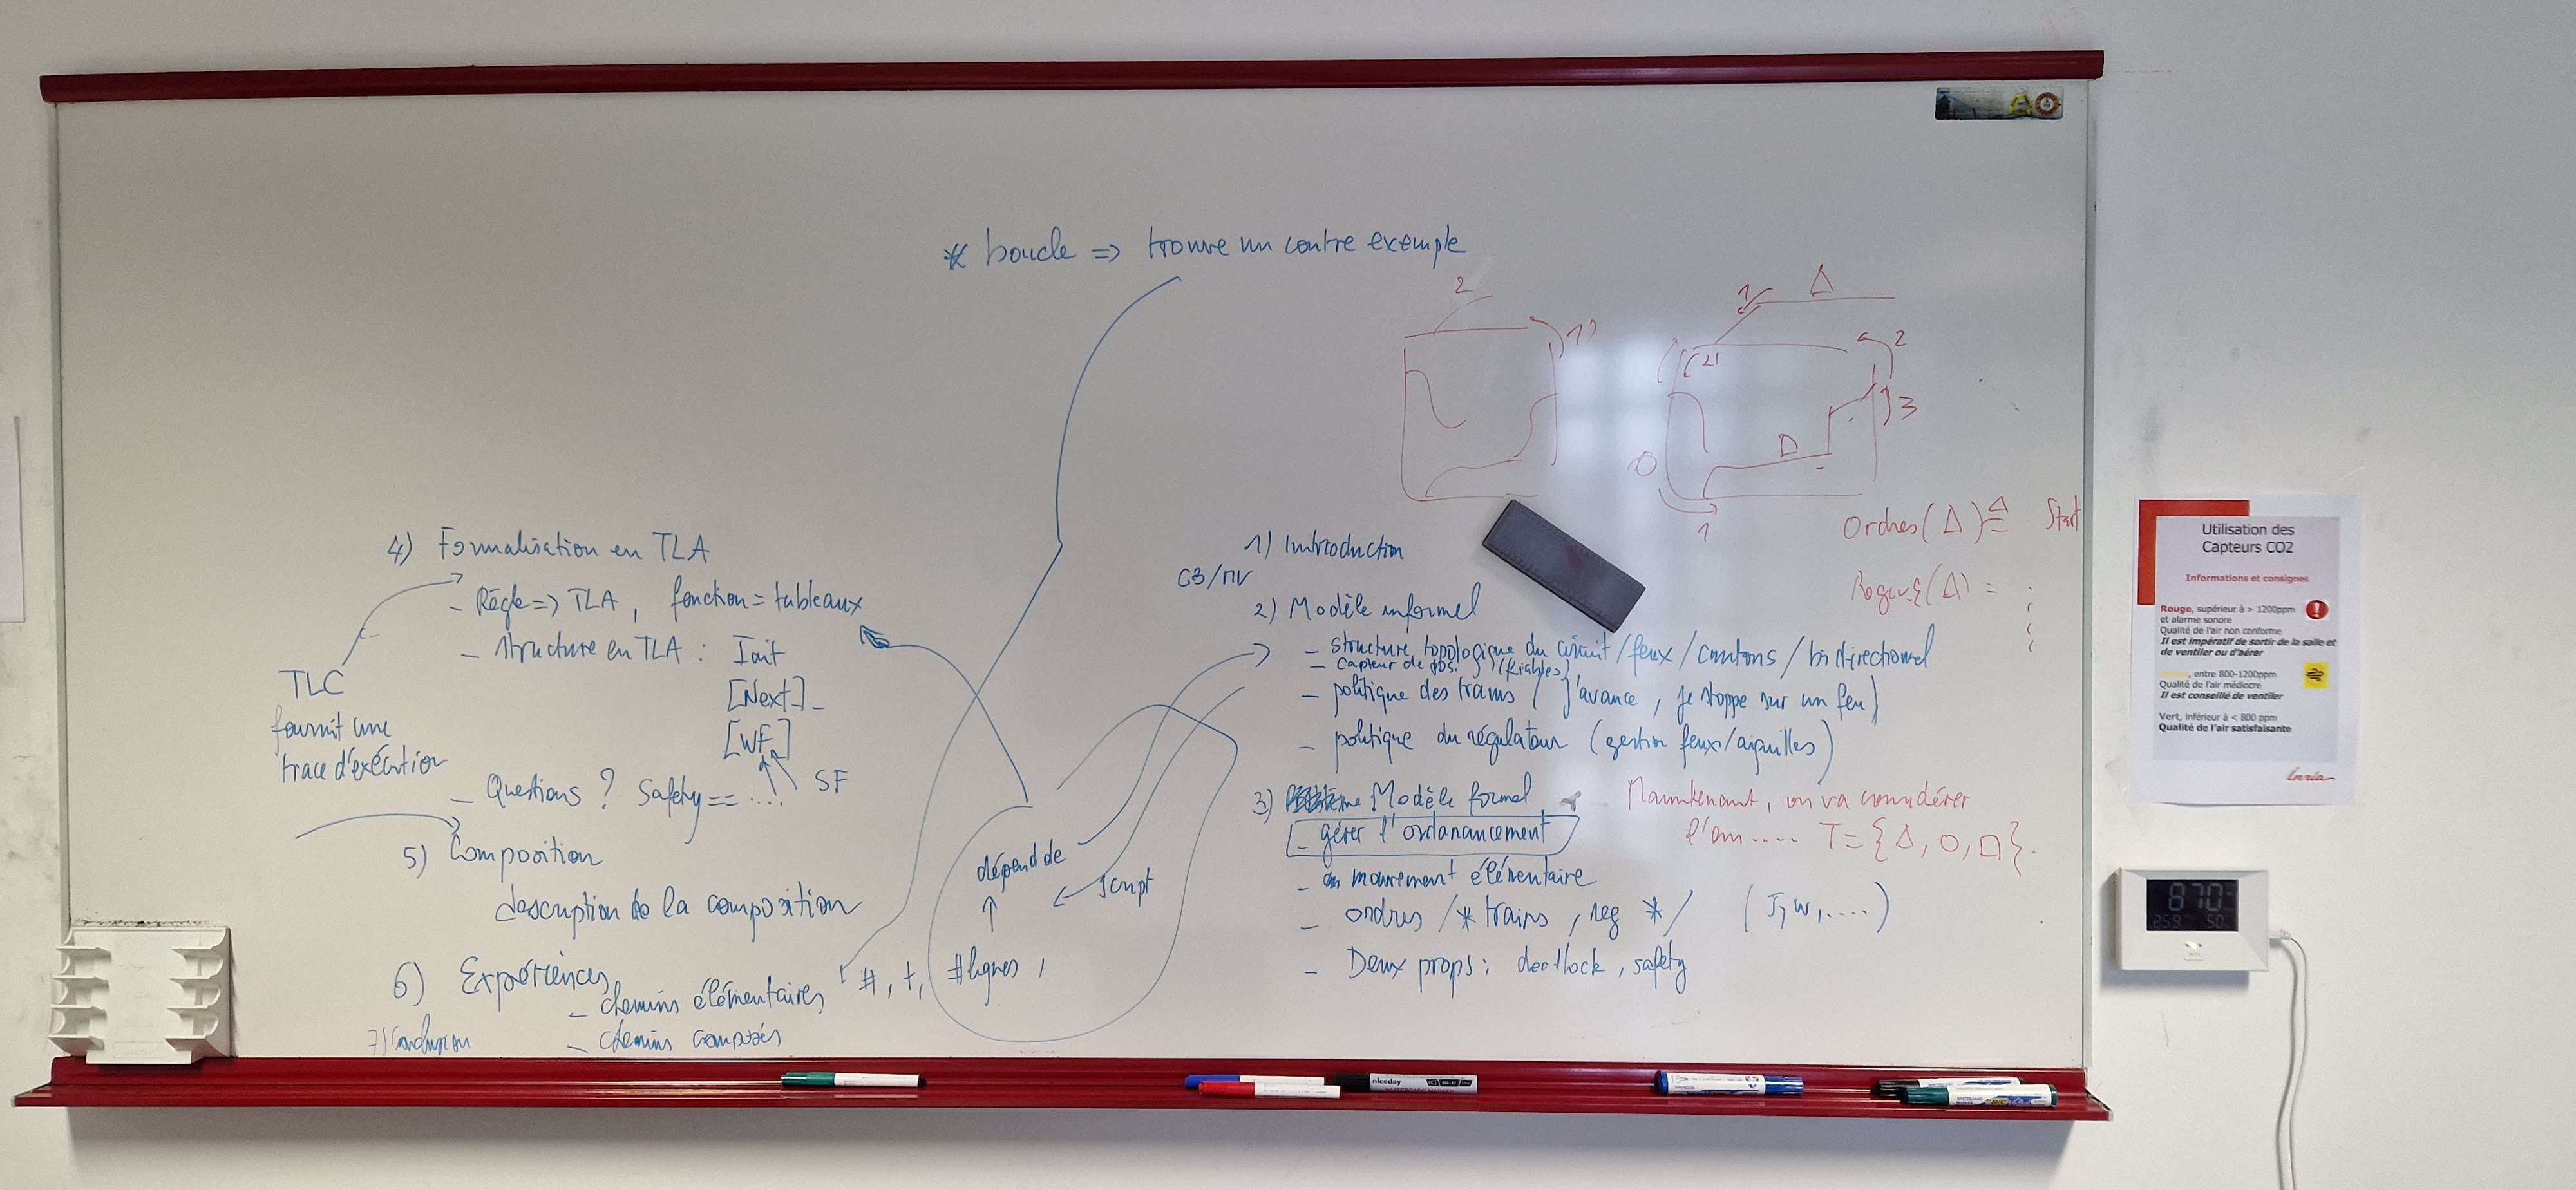
\includegraphics[scale=0.1]{img/sommaire_tableau.jpg}

\paragraph{Acknowledgements} The authors would like to thank Sébastien Schmitt from CNRS who built the train model mentioned in the introduction. That gave us a concrete reason to think about routes, scheduling and proofs. 

\bibliographystyle{splncs04}
\bibliography{refs}
\end{document}
